\chapter{Υλοποίηση συστήματος Μηχανικής Μάθησης}

Αυτό το κεφάλαιο περιγράφει την διαδικασία σχεδιασμού και υλοποίησης των μοντέλων που αναπτύχθηκαν με σκοπό την παραγωγή επιπέδων, παρόμοιων χαρακτηριστικών, με τα επίπεδα που αναλύθηκαν στον κεφάλαιο 2. Η υλοποίηση είναι μια εφαρμογή Machine Learning Content Generation (MLCG). Αποτελεί μια απόδειξη, από την θεωρία στην πράξη της υπόθεσης ότι μοντέλα Deep Neural Networks και συγκεκριμένα GANs \cite{firstgan3} \cite{firstgan} \cite{firstgan2} μπορούν να χρησιμοποιηθούν με επιτυχία για την κατασκευή περιεχομένου.
\par
Η υλοποίηση περιλάμβανε την ολοκλήρωση πολλών επιμέρους κομματιών, κάποια από τα οποία δεν χρησιμοποιήθηκαν τελικά στην εκπαίδευση του τελικού μοντέλου. Κάτι το οποίο είναι συχνό και αναμενόμενο όταν υλοποιούνται εφαρμογές τέτοιας πολυπλοκότητας. Για παράδειγμα υλοποιήθηκαν μέθοδοι που πρόσθεταν θόρυβο στις διακριτές τιμές της εισόδου ώστε να μετατρέπονται σε συνεχείς τιμές με κανονική κατανομή. Αυτό το κομμάτι αποδείχθηκε ότι τελικά δεν προσφέρει στην απόδοση του συστήματος οπότε δεν χρησιμοποιείται στα τελικά αποτελέσματα, που θα αναλυθούν. Παραμένει κομμάτι της υλοποίησης χωρίς όμως να συνεισφέρει στο τελικό αποτέλεσμα.

\section{Τεχνική περιγραφή}
Το σύστημα MLCG αναπτύχθηκε στην γλώσσα \textit{Python}, μια από τις πιο διαδεδομένες γλώσσες για υλοποιήσεις Μηχανικής Μάθησης. Η έκδοση που χρησιμοποιήθηκε είναι η 3.7. Επιλέχθηκε η συγκεκριμένη έκδοση καθώς είναι η πιο πρόσφατη έκδοση της γλώσσας, που υποστηρίζει τις βιβλιοθήκες για Deep Neural Networks που χρησιμοποιήθηκαν. 
Μερικές από τις πιο σημαντικές βιβλιοθήκες και εργαλεία που χρησιμοποιήθηκαν:

\begin{description}
\item[$\bullet$ Numpy] Βιβλιοθήκη για επιστημονικές εφαρμογές και υπολογισμούς της γλώσσας Python.
\item[$\bullet$ Matplotlib] Βιβλιοθήκη για την οπτικοποίηση αποτελεσμάτων και μετρικών.
\item[$\bullet$ Tensorflow] Αποτελεί ένα ολοκληρωμένο σύστημα για εφαρμογές Machine Learning με υποστήριξη για πολλές γλώσσες προγραμματισμού. 
\item[$\bullet$ Keras] Αποτελεί την βιβλιοθήκη σε Python, για την χρησιμοποίηση του συστήματος Tensorflow σε εφαρμογές ανεπτυγμένες σε αυτή την γλώσσα.
\item[$\bullet$ Tensorboard] Μια βιβλιοθήκη οπτικοποίησης των αποτελεσμάτων εκπαίδευσης και αρχιτεκτονικής που χρησιμοποιείται σε συνδυασμό με την βιβλιοθήκη \textit{Tensorflow}. 
\end{description}


\section{Δεδομένα εκπαίδευσης}
Όπως αναλύθηκε και στο κεφάλαιο σχετικά με την υλοποίηση του PCG συστήματος σε Python, το dataset αποτελείται από αρχεία κειμένου, όπου το κάθε αρχείο αντιστοιχεί σε ένα επίπεδο. Για την εκπαίδευση του μοντέλου, δημιουργήθηκε ένα \textit{dataset} που περιλαμβάνει 1000 τέτοια αρχεία.
\par
Όπως σε όλες τις εφαρμογές Μηχανικής Μάθησης, τα δεδομένα του dataset δεν δίνονται απευθείας στο μοντέλο για εκπαίδευση αλλά περνάνε από διάφορες μεθόδους προεργασίας ώστε να εξασφαλίσουμε καλύτερα και πιο αξιόπιστα αποτελέσματα.


\subsection{Χαρακτηριστικά του dataset}
Το κάθε επίπεδο είναι ένας πίνακας \textit{10000} στοιχείων, όπου το κάθε στοιχείο αντιστοιχεί σε ένα κελί στην 100x100 grid απεικόνιση του επιπέδου. Μόλις το PCG σύστημα δημιουργεί ένα επίπεδο, το μετατρέπει στην αναπαράσταση του αρχείου και το αποθηκεύει ώστε να μπορεί να διαβαστεί από το σύστημα Μηχανικής Μάθησης.
\par
Απόσπασμα από αρχείο του dataset:
\begin{verbatim}
100, 100
Tile X,Tile Y,Tile Type
0,0,1
0,1,1
0,2,1
0,3,1
0,4,1
0,5,1
\end{verbatim}
Στο παραπάνω παράδειγμα βλέπουμε τις πρώτες γραμμές από ένα αρχείο επιπέδου. Η πρώτη σειρά δηλώνει το μέγεθος του επιπέδου, κάτι το οποίο προστέθηκε για πληροφοριακούς λόγους αλλά δεν χρησιμοποιείται από το MLCG. Η δεύτερη σειρά αναγράφει το είδος των στοιχείων που αντιστοιχούν στην κάθε κολόνα αντίστοιχα.
\par

\begin{itemize}
\item Η πρώτη κολόνα, Tile X, δηλώνει την x συντεταγμένη του στοιχείου μέσα στο επίπεδο.
\item Η δεύτερη κολόνα, Tile Y, δηλώνει την y συντεταγμένη του στοιχείου μέσα στο επίπεδο.
\item Η τρίτη κολόνα, Tile Type, δηλώνει το είδος του στοιχείου \textit{(Wall, Room)} με ένα διακριτό ακέραιο αριθμό \textit{(0, 1)} αντίστοιχα.
\end{itemize}

\par
H αρίθμηση των στοιχείων μέσα στο grid ξεκινάει από την κάτω αριστερή γωνία, αυτό είναι το στοιχείο με συντεταγμένες 0,0 και προχωράει πρώτα στον κάθετο άξονα (Υ) και στη συνέχεια στον οριζόντιο άξονα (Χ). Το τελευταίο στοιχείο που αναγράφετε με συντεταγμένες 99,99 αντιστοιχεί στην πάνω δεξιά γωνία του grid.

\subsection{Προ επεξεργασία Δεδομένων}
Πριν από το στάδιο της εκπαίδευσης, τα δεδομένα που θα εισάγουμε στο σύστημα πρέπει να περάσουν από το στάδιο της προ επεξεργασίας ώστε να πληρούν κάποιες προϋποθέσεις.
\par
Σε αυτή την εφαρμογή έχουμε δύο ειδών τιμές που μπορεί να λάβει ένα στοιχείο \textit{(Wall, Room)} τα οποία είναι αντίστοιχα οι αριθμοί \textit{(0, 1)}. Ως προ επεξεργασία των δεδομένων εφαρμόζετε \textit{One hot encoding} στα δεδομένα μας το οποίο λαμβάνει μια διακριτή τιμή και την μετατρέπει σε ένα διάνυσμα τιμών. Το διάνυσμα αυτό έχει ένα \textit{1} και όλα τα υπόλοιπα στοιχεία \textit{0}.
\par
Για παράδειγμα, στην περίπτωση της εφαρμογής το στοιχείο με αριθμό \textit{0} θα μετατραπεί στο διάνυσμα \textit{(1, 0)} και αντίστοιχα το στοιχείο  με αριθμό \textit{1} θα μετατραπεί στο διάνυσμα \textit{(0, 1)}. 
\par
To \textit{One hot encoding} συνίσταται σε εφαρμογές που δεν έχουν πολλές διακριτές τιμές τα δεδομένα τους, όπως σε αυτή την εφαρμογή.

\par
Το δεύτερο κομμάτι αφορά το είδος του μοντέλου που θέλουμε να εκπαιδεύσουμε. Στην υλοποίηση της εργασίας αναπτύχθηκε ένα μοντέλο GAN, το Convolutional επειδή αποτελείται κυρίως από επίπεδα συνέλιξης (\textit{convolution}). Το μοντέλο ανάλογα με τα επιπέδων που έχει, δέχεται την είσοδο σε διαφορετική μορφή από αυτήν στην οποία είναι αποθηκευμένα τα επίπεδα. Το Convolutional μοντέλο δέχεται ως είσοδο θόρυβο, ένα διάνυσμα (100, 1) τυχαίων αριθμών, και παράγει ως έξοδο ένα πίνακα (100, 100) στοιχείων.
\par


\section{Επεξεργασία Αποτελεσμάτων}
Η αντίθετη διαδικασία πρέπει να εκτελεστεί για τα αποτελέσματα του μοντέλου GAN. Τα αποτελέσματα του Convolutional μοντέλου πρέπει να μετατραπούν σε διάνυσμα (10000, 1) για να αποθηκευτούν με την μορφή που έχει όλο το dataset.
\par
Επίσης τα αποτελέσματα είναι σε \textit{One hot encoding} αναπαράσταση και πρέπει να γίνει η μετατροπή τους αντίστοιχη διακριτή τιμή από τις διαθέσιμες [0, 1]. Τα αποτελέσματα του Gan δεν είναι σε απόλυτες τιμές (0, 1) ακόμα και στην \textit{One hot encoding} αναπαράσταση, αλλά έχουν τις τιμές των πιθανοτήτων που προέβλεψε το μοντέλο για το κάθε στοιχείο του διανύσματος. 
\par
Για παράδειγμα μπορεί ένα στοιχείο να προβλεφτεί από το μοντέλο ως \textit{(0.6, 0.4)}, σε αυτή την περίπτωση μετατρέπουμε την μεγαλύτερη πιθανότητα σε \textit{(1)} και όλες τις υπόλοιπες σε \textit{(0)}. Συνεπώς το παράδειγμα θα γίνει \textit{(1, 0)} το οποίο αντίστοιχα θα μεταφραστεί ως \textit{(0)} με βάση την αντιστροφή της αρχικής διαδικασίας του \textit{One hot encoding}.


\subsection{Δειγματοληψία κατά την εκπαίδευση}
Για να παρακολουθούμε την πρόοδο της εκπαίδευσης ανά τακτές χρονικές περιόδους, ορίστηκε μια μεταβλητή που δηλώνει ανά πόσες εποχές, θα γίνετε δειγματοληψία από το μοντέλο. Επίσης μια τελική δειγματοληψία γίνετε μόλις ολοκληρωθούν όλες οι εποχές της εκπαίδευσης ώστε να έχουμε δείγμα από το τελικό μοντέλο. 
\par
Σε κάθε δειγματοληψία, το μοντέλο εκτελείται με μια είσοδο εκπαίδευσης και με βάση τα βάρη που έχει εκείνη την στιγμή. Το αποτέλεσμα περνάει από την επεξεργασία που αναλύθηκε παραπάνω και αποθηκεύεται σε ένα αρχείο με όνομα που να εκφράζει το στάδιο της εκπαίδευσης στο οποίο βρισκόταν το νευρωνικό όταν δημιουργήθηκε αυτό το δείγμα.
\par
Για παράδειγμα το αρχείο \verb|combined_1000_09-03-2020_21-11-56FGAE.csv| είναι ένα δείγμα που δημιουργήθηκε από τον Generator σε συνεργασία με τον Discriminator (\textit{combined}) στην εποχή 1000 της εκπαίδευσης. Τα υπόλοιπα στοιχεία δηλώνουν την ημερομηνία που εκτελέστηκε η συγκεκριμένη εκπαίδευση. Στο τέλος του κάθε ονόματος προστίθεται και ένα τυχαίο αλφαριθμητικό. 
\par
Το μοντέλο που δημιούργησε αυτό το δείγμα αναφέρεται στον φάκελο που είναι αποθηκευμένο \verb|cnn_gan-09_03_2020_21_08_34|. Αυτή η ονοματολογία δηλώνει το μοντέλο (\textit{cnn} και στην συνέχεια ακολουθεί η ημερομηνία και η ώρα που ξεκίνησε η εκπαίδευση του συγκεκριμένου μοντέλου.

\subsection{Αποθήκευση μοντέλου}
Το κάθε μοντέλο μόλις εκπαιδευτεί, αποθηκεύεται σε αρχεία από τα οποία είναι δυνατή η φόρτωση του στην κατάσταση που ήταν μόλις τελείωσε η εκπαίδευση. Συγκεκριμένα αποθηκεύεται η αρχιτεκτονική και τα βάρη του μοντέλου, σε ειδικά αρχεία ώστε να μπορούμε οποιαδήποτε στιγμή να τα φορτώσουμε και να τα εκτελέσουμε. Η αποθήκευση γίνεται μέσα στον φάκελο του μοντέλου, που δημιουργείται μόλις ξεκινήσει η εκπαίδευση.
\par
Μέσα στον φάκελο του μοντέλου αποθηκεύονται:
\begin{description}
\item[$\bullet$ Χαρακτηριστικά του μοντέλου] Όλη η αρχιτεκτονική του μοντέλου, τα επίπεδα, ο αριθμός και το είδος των παραμέτρων του κάθε επιπέδου, για το δίκτυο του Generator και του Discriminator. Αυτά αποθηκεύονται μέσα στον φάκελο \texttt{model\_data} στα αρχεία  \textit{generator.json} και \textit{discriminator.json} αντίστοιχα.
\item[$\bullet$ Τα βάρη του μοντέλου] Σε αντίστοιχα αρχεία \textit{generator.h5} και \textit{discriminator.h5} αποθηκεύονται τα βάρη του κάθε δικτύου.
\item[$\bullet$ Μετρικές και αποτελέσματα] Στο αρχείο \textit{results.txt} αποθηκεύονται οι τελικές μετρήσεις και αποτελέσματα της απόδοσης του κάθε μοντέλου μαζί με διάφορες παραμέτρους που έχουμε ορίσει για την εκπαίδευση και τις τιμές τους. Με αυτό τον τρόπο μπορούμε εύκολα να συγκρίνουμε τα διάφορα μοντέλα.
\item[$\bullet$ Επίπεδα που παράχθηκαν] Στον φάκελο \textit{Results} αποθηκεύονται τα επίπεδα που δημιουργήθηκαν με την δειγματοληψία που αναφέραμε παραπάνω.
\item[$\bullet$ Εικόνες επιπέδων] Τα επίπεδα που δημιουργούνται μέσω της δειγματοληψίας, αποτυπώνονται και σε εικόνες για την άμεση παρακολούθηση και αξιολόγηση της εκπαίδευσης όσο εκτελείται και για την σύγκριση αποτελεσμάτων μεταξύ εκπαιδεύσεων. Αυτές οι εικόνες αποθηκεύονται στον φάκελο \textit{Images} του κάθε μοντέλου.
\item[$\bullet$ Αρχεία Tensorboard] Τα αρχεία με τα αποτελέσματα της εκπαίδευσης, και την αρχιτεκτονική των μοντέλων τα οποία μπορούν να χρησιμοποιηθούν από την βιβλιοθήκη του Tensorboard, αποθηκεύονται στον φάκελο \textit{com\_logs}. Από αυτά τα αρχεία μπορούν να παραχθούν γραφήματα και μετρικές σχετικά με την πρόοδο του μοντέλου.
\end{description}

\subsection{Αρχιτεκτονική Generator}
Το μοντέλο του Generator δικτύου, αποτελείται από 22 επίπεδα συνολικά. Από αυτά ξεχωρίζουμε τα επίπεδα εισόδου και εξόδου που έχουν ως ρόλο να μετατρέψουν την μορφή που έχουν τα δεδομένα και τα επίπεδα επεξεργασίας που αποθηκεύουν και επεξεργάζονται την πληροφορία που αναπαριστούν τα επίπεδα. Παρατηρούμε ότι υπάρχει ένα κοινό μοτίβο στα επίπεδα επεξεργασίας, όπου βλέπουμε αρχικά να υπάρχει ένα επίπεδο που εκτελεί κάποια επεξεργασία στα δεδομένα, όπως το επίπεδο \textit{Conv2DTranspose} και στη συνέχεια ένα επίπεδο κανονικοποίησης των τιμών που παράχθηκαν \textit{BatchNormalization} και φιλτραρίσματος των αποτελεσμάτων \textit{LeakyReLU}.

% Dense
\begin{description}
\item[$\bullet$ Dense επίπεδο] Το Dense επίπεδο λαμβάνει ως είσοδο τον θόρυβο που έχουμε δημιουργήσει ως διάνυσμα (100, 1) στοιχείων, παίρνει ως είσοδο, και εφαρμόζει τη συνάρτηση εσωτερικού γινομένου στα στοιχεία εισόδου με στόχο να δημιουργήσει \textit{units} καινούργιες διαστάσεις με τα αποτελέσματα. Ο αριθμός \textit{units} ορίζετε σε κάθε Dense επίπεδο. Για παράδειγμα για το επίπεδο εισόδου του generator ορίζουμε:
\begin{verbatim}
units = 25 * 25 * depth
self.add_layer(Dense(units, input_dim=self.latent_dim))
\end{verbatim}
\par
Το παραπάνω επίπεδο έχει είσοδο ένα διάνυσμα (100, 1) και ως έξοδο ένα διάνυσμα (25 * 25 * depth, 1) όπου το \textit{depth} κατά την εκπαίδευση ορίστηκε ως 64. \cite{dense}
\end{description}

% LeakyReLU
\begin{description}
\item[$\bullet$ LeakyReLU] Αυτό το επίπεδο είναι μια παραλλαγή του επιπέδου \textit{ReLU} που αναλύσαμε. Η διαφορά  του επιπέδου LeakyReLU είναι ότι στην περίπτωση μη ενεργοποίησης του επιπέδου από την είσοδο, η έξοδος δεν είναι μηδενική όπως στο επίπεδο της \textit{ReLU} αλλά επιστρέφει ως έξοδο μια πολύ μικρή τιμή, γιαυτό και λέγεται \textit{LeakyReLU}(διαρροή). Η συνάρτηση ενεργοποίησης της LeakyReLU ορίζετε ως:
\par
$f(x) = alpha * x,  \;\; if \;\; x < 0$
\par
$f(x) = x,  \;\; if \;\; x >= 0$
\par
To alpha είναι μια παράμετρος που μπορεί να οριστεί σε κάθε επίπεδο LeakyReLU. Στην συγκεκριμένη υλοποίηση ορίστηκε ως εξής:
\begin{verbatim}
LeakyReLU(alpha=0.2)
\end{verbatim}
\par
O ορισμός του alpha με την τιμή 0.2 έγινε μετά από έρευνα σε αντίστοιχες υλοποιήσεις και παρατηρήσεις κατά την εκπαίδευση. \cite{firstgan} \cite{firstgan2} \cite{firstgan3} \cite{leakyrelu}
\end{description}

% BatchNormalization
\begin{description}
\item[$\bullet$ BatchNormalization] To επίπεδο του BatchNormalization όπως αναφέρει και το όνομα κανονικοποιεί την είσοδο που δέχεται. To επίπεδο Dropout απενεργοποιεί τυχαία κάποιες από τις εξόδους μετατρέποντας τις τιμές τους σε 0. \cite{batch}
\par
\begin{verbatim}
BatchNormalization(momentum=0.8)
Dropout(rate=0.3)
\end{verbatim}
\par
Η παράμετρος momentum χρησιμοποιείται με την τιμή 0.8 για να βελτιώσει την απόδοση του νευρωνικού και να αυξήσει την ταχύτητα της εκπαίδευσης \cite{firstgan}.
\end{description}

% Dropout
\begin{description}
\item[$\bullet$ Dropout] To επίπεδο Dropout απενεργοποιεί τυχαία κάποιες από τις εξόδους μετατρέποντας τις τιμές τους σε 0. \cite{dropout}
\par
\begin{verbatim}
Dropout(rate=0.3)
\end{verbatim}
\par
H παράμετρος rate δηλώνει το ποσοστό επί τις εκατό των τιμών που θα γίνουν 0 στο επίπεδο Dropout.
\end{description}

% Reshape
\begin{description}
\item[$\bullet$ Reshape] To επίπεδο Reshape μετατρέπει τα δεδομένα σε μια συγκεκριμένη μορφή χωρίς να εφαρμόζει καμία επεξεργασία πάνω τους. Χρησιμοποιείται συνήθως για να προετοιμάσει δεδομένα σε μορφή πίνακα ώστε να εισαχθούν σε επίπεδα με συνέλιξη. \cite{reshape}
\par
\begin{verbatim}
Reshape(target_shape=(25, 25, depth))
\end{verbatim}
\end{description}

% Conv2DTranspose
\begin{description}
\item[$\bullet$ Conv2DTranspose επίπεδο] H πράξη που εφαρμόζετε από αυτό το επίπεδο είναι η αντίστροφη διαδικασία από αυτήν της συνέλιξης \textit{Deconvolution}. \cite{conv2dtranspose}
\begin{verbatim}
Conv2DTranspose(int(depth/2), 5, padding='same')
\end{verbatim}
\par
Το πρώτο όρισμα είναι ο αριθμός των φίλτρων που θα παραχθούν, το δεύτερο όρισμα είναι το μέγεθος του \textit{kernel} που θα χρησιμοποιηθεί (5,5) και το είδος του padding που θα εφαρμοστεί.
\end{description}

% UpSampling2D
\begin{description}
\item[$\bullet$ UpSampling2D επίπεδο] Αυξάνει το μέγεθος των δεδομένων με το να επαναλαμβάνει σειρές και στήλες από την είσοδο. \cite{upsampling2d}
\begin{verbatim}
UpSampling2D() 
\end{verbatim}
\par
\end{description}

Αρχιτεκτονική μοντέλου:
\begin{verbatim}
        
depth = 64
units = 25 * 25 * depth
        
Dense(units, input_dim=self.latent_dim)
BatchNormalization(momentum=0.8)
LeakyReLU(0.2)

# Reshape to 25 x 25 x depth
Reshape(target_shape=(25, 25, depth))
Dropout(0.3)

# Upsample to 50 x 50 x depth
UpSampling2D()

# Change to 50 x 50 x depth / 2
Conv2DTranspose(int(depth/2), 5, padding='same')
BatchNormalization(momentum=0.8)
LeakyReLU(0.2)

# Upsample to 100 x 100 x depth / 2
UpSampling2D()

# Change to 100 x 100 x depth / 4
Conv2DTranspose(int(depth/4), 5, padding='same')
BatchNormalization(momentum=0.8)
LeakyReLU(0.2)

# Change to 100 x 100 x 2
        
Conv2DTranspose(2, 5, padding='same')
BatchNormalization(momentum=0.8)
LeakyReLU(0.2)
\end{verbatim}

\begin{figure}[H]
\centering
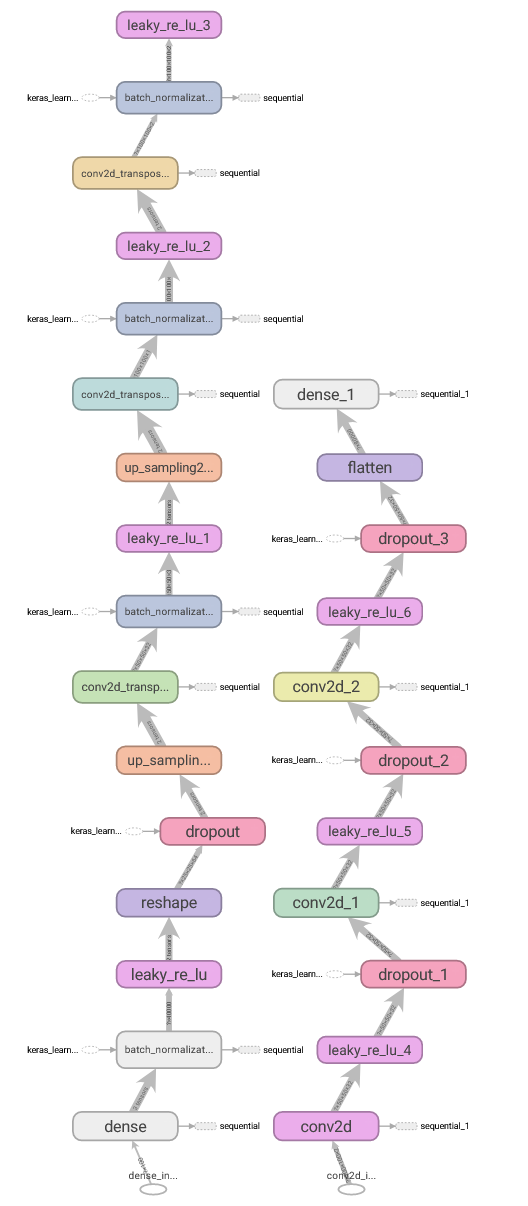
\includegraphics[width=.8\linewidth]{../images/graphs/tb-model-graph.png}
\label{fig:fig}
\end{figure}

\addtocounter{figure}{-1}
\begin{figure} [H]
\caption{Γραφική απεικόνιση των επιπέδων του Generator(αριστερά) και του Discriminator(δεξιά). Η εικόνα προέρχεται από το Tensorboard.}
\end{figure}


\subsection{Αρχιτεκτονική Discriminator}
Το μοντέλο του Discriminator δικτύου, είναι πολύ πιο μικρό από το μοντέλο του Generator. Αποτελείται από μόλις 11 επίπεδα. Η είσοδος του δικτύου είναι ένα επίπεδο διανυσματικής μορφής με τις διαστάσεις και τις τιμές ενός επιπέδου και έχει ως έξοδο μία τιμή στο διακριτό διάστημα [0, 1].
\newline
Τα επίπεδα του Discriminator όπως ορίζονται στην υλοποίηση:
\begin{verbatim}
Conv2D(32, 3, padding='same', strides=2,input_shape=self.dungeon_shape)
LeakyReLU(0.2)
Dropout(0.3)

Conv2D(32, 3, padding='same', strides=1)
LeakyReLU(0.2)
Dropout(0.3)

Conv2D(32, 3, padding='same', strides=1)
LeakyReLU(0.2)
Dropout(0.3)

Flatten()
Dense(1, activation='sigmoid')
\end{verbatim}

\par
To επίπεδο της εξόδου παράγει μία τιμή με συνάρτηση ενεργοποίησης την σιγμοειδή (\textit{sigmoid}) συνάρτηση, ώστε να έχουμε το αποτέλεσμα μεταξύ 0 και 1. Όπου το 0 και τιμές κοντά στο 0 δηλώνουν ότι το επίπεδο αποτελεί δημιούργημα του Generator και όχι κάποιο από τα δείγματα εκπαίδευσης και το 1 δηλώνει ότι το επίπεδο είναι από τα δείγματα εκπαίδευσης ή μοιάζει τόσο πολύ που δεν μπορεί να το ξεχωρίσει από τα "πραγματικά".


\section{Εκπαίδευση GAN}
Το dataset που χρησιμοποιήθηκε κατά την εκπαίδευση αποτελείται από 1000 αρχεία όπου το κάθε αρχείο αντιστοιχεί σε ένα επίπεδο. Πριν ξεκινήσει η διαδικασία την εκπαίδευσης, φορτώνονται όλα τα επίπεδα στην μνήμη και περνάνε από το στάδιο της προ επεξεργασίας για να έρθουν σε μορφή που να μπορούν να επεξεργαστούν το GAN.
\par

\begin{figure}[H]
\centering
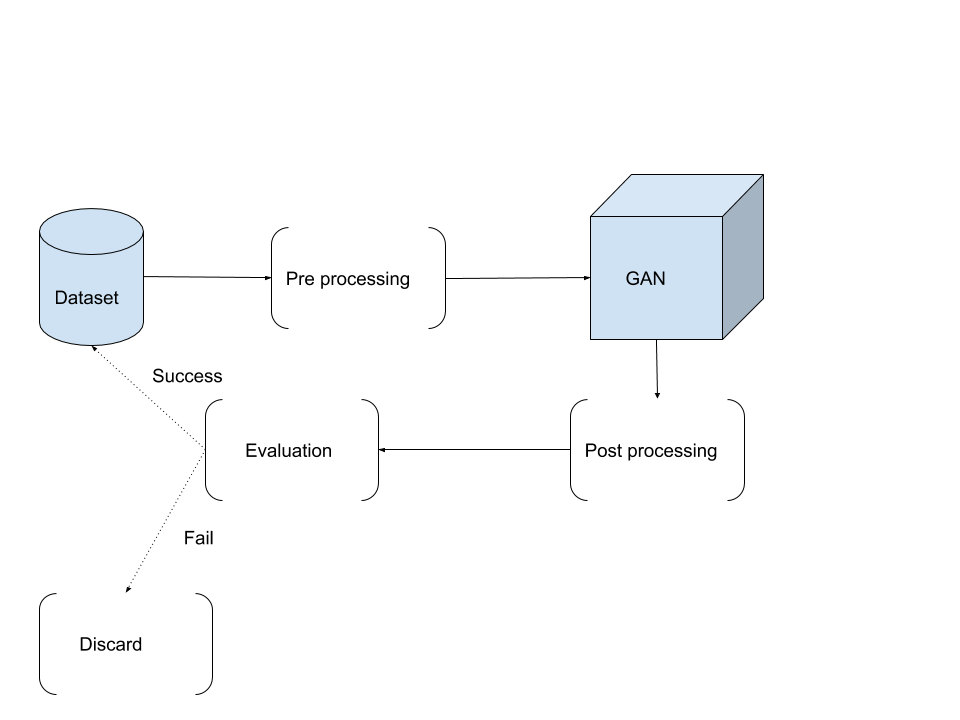
\includegraphics[width=.8\linewidth]{../images/graphs/Abstract_functionality.png}
\caption{Αναπαράσταση εκπαίδευσης ενός μοντέλου GAN}
\label{fig:fig}
\end{figure}

\subsection{Μεταβλητές εκπαίδευσης}
Κατά την δημιουργία του μοντέλου ορίζονται μεταβλητές που θα χρησιμοποιηθούν στο στάδιο της εκπαίδευσης. Όλες οι μεταβλητές έχουν προ ρυθμισμένες τιμές οι οποίες βγήκαν μέσα από δοκιμές. Μερικές από τις πιο σημαντικές είναι:


\begin{description}
\item[$\bullet$ epochs] Θετικός ακέραιος αριθμός που ορίζει τον αριθμό των εποχών που θα επαναληφθεί η εκπαίδευση. Η προτεινόμενη τιμή του για αυτή την υλοποίηση είναι 2000.
\item[$\bullet$ batch\_size] Θετικός ακέραιος αριθμός που ορίζει τον αριθμό των δειγμάτων που θα δίνονται σε κάθε εποχή για εκπαίδευση. Εάν το batch\_size είναι μικρότερο του μεγέθους του dataset, τα δείγματα που θα συμμετέχουν στην εκπαίδευση επιλέγονται τυχαία με δειγματοληψία σε κάθε εποχή και χωρίς επανατοποθέτηση. Στην περίπτωση που το batch\_size είναι μεγαλύτερο του μεγέθους του dataset, ορίζετε ως batch\_size το μέγεθος του dataset. Η προτεινόμενη τιμή του για αυτή την υλοποίηση είναι 700.
\item[$\bullet$ sample] Θετικός ακέραιος αριθμός που ορίζει το διάστημα ανάμεσα στις εποχές που λαμβάνουμε ένα δείγμα επιπέδου από το μοντέλο σε εκείνο το στάδιο της εκπαίδευσης. Αυτή η μεταβλητή ορίστηκε για να μπορούμε να παρακολουθούμε την πρόοδο του δικτύου όσο εκπαιδεύεται. Η προτεινόμενη τιμή του για αυτή την υλοποίηση είναι 50.
\end{description}

\subsection{Είσοδος εκπαίδευσης Generator}
Το μοντέλο του Generator δέχεται ως είσοδο ένα διάνυσμα 100 στοιχείων θορύβου. Από αυτόν τον θόρυβο θα παράξει ένα επίπεδο (100, 100) στοιχείων. O Generator εκπαιδεύεται πάντα μαζί με τον Discriminator κατά την εκπαίδευση ολόκληρου του μοντέλου GAN.

\subsection{Λειτουργία Generator}
Για την λειτουργία του Generator, εκτός του σταδίου της εκπαίδευσης, πρέπει να του δώσουμε ως είσοδο ένα δείγμα θορύβου για να δημιουργήσει ένα δείγμα επιπέδου.

\subsection{Είσοδος εκπαίδευσης Discriminator}
Για την εκπαίδευση του Discriminator δίνουμε ως είσοδο έναν πίνακα και ένα διάνυσμα. Ο πίνακας περιέχει τα δείγματα που θέλουμε να αξιολογήσει ως "τεχνητά" από τον Generator ή "πραγματικά" από το dataset. Το διάνυσμα έχει δυαδικές τιμές που δηλώνουν την πραγματική προέλευση του κάθε δείγματος με τις τιμές 0 και 1.
\par
Για να εκπαιδευτεί ο Discriminator παίρνει ως είσοδο τα επίπεδα και ελέγχει την έξοδο του εάν ταιριάζει με την αντίστοιχη τιμή για αυτό το επίπεδο με το διάνυσμα των πραγματικών τιμών. Ομοίως διορθώνει τα βάρη του στις περιπτώσεις λάθους εάν έχουμε ενεργοποιήσει την μεταβλητή train\_discriminator.

\section{Εκπαίδευση μοντέλου GAN}
\par
Η εκπαίδευση του GAN μοντέλου, γίνεται σε δύο στάδια. Στο πρώτο στάδιο εκπαιδεύεται το μοντέλο του Discriminator με το υπάρχον dataset και με επίπεδα που παράγει ο Generator όπως είναι σε εκείνο το στάδιο. Στο πρώτο στάδιο έχουμε επισημάνει τα επίπεδα ανάλογα με το εάν ανήκουν στο dataset ή είναι δημιουργημένα από τον Generator ώστε ο Discriminator να μπορέσει να διορθώσει τα βάρη του αντίστοιχα.
\par
Στο δεύτερο στάδιο, εκπαιδεύουμε το μοντέλο του GAN το οποίο περιέχει τον Generator και τον Discriminator μαζί αλλά τα επίπεδα του Discriminator δεν ανανεώνουν τα βάρη τους σε κάθε εποχή, αντίθετα γυρνάνε το λάθος κατευθείαν στον Generator ώστε να ενημερώσει μόνο αυτός τα βάρη του και να εκπαιδευτεί. Στο δεύτερο στάδιο προσομοιώνουμε έναν τέλειο Discriminator ο οποίος αναγνωρίζει όλα τα επίπεδα που έχουν δημιουργηθεί από τον Generator και κατά συνέπεια γίνετε συνέχεια διόρθωση βαρών για τον Generator.
\par
Το κάθε στάδιο επαναλαμβάνετε για ένα συγκεκριμένο αριθμό από εποχές κάθε φορά και στην συνέχεια το επόμενο στάδιο ξεκινάει και εκτελείται για τον ίδιο αριθμό από εποχές. Μόλις εκτελεστούν και τα δύο στάδια για τον συνολικό αριθμό εποχών που έχουμε ορίσει, η εκπαίδευση σταματάει.
\par
Παρατηρούμε ότι το μοντέλο του Generator δεν εκπαιδεύεται απευθείας και δεν λαμβάνει ποτέ ως ανατροφοδότηση κάποιο πραγματικό επίπεδο, αντίθετα όλη η πληροφορία που λαμβάνει προέρχεται από τον Discriminator και μέσω των μοτίβων που έχει μάθει να αναγνωρίζει περνάει η πληροφορία του επιπέδου και στον Generator.


\section{Αποτελέσματα}

\subsection{Αποτελέσματα του Generator και του Discriminator του CNN δικτύου}
\begin{figure}[H]
\begin{subfigure}{.5\textwidth}
  \centering
  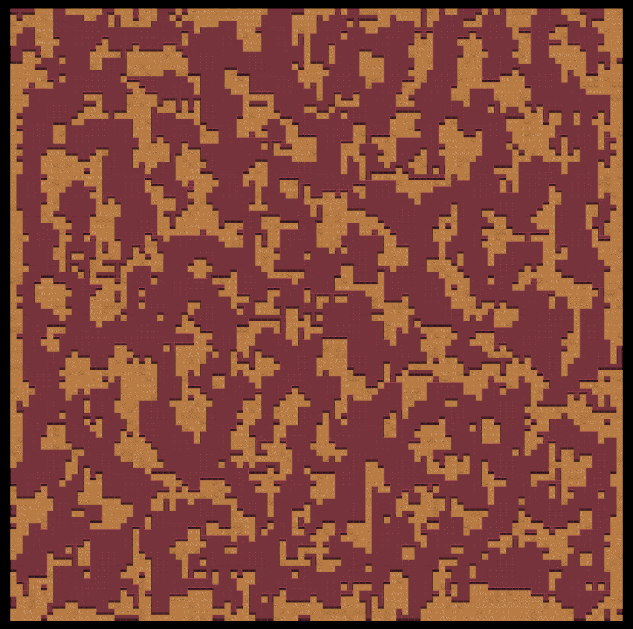
\includegraphics[width=.8\linewidth]{../images/generated/50.png}
  \caption{Επίπεδο μετά από 50 εποχές}
  \label{fig:sfig1}
\end{subfigure}%
\begin{subfigure}{.5\textwidth}
  \centering
  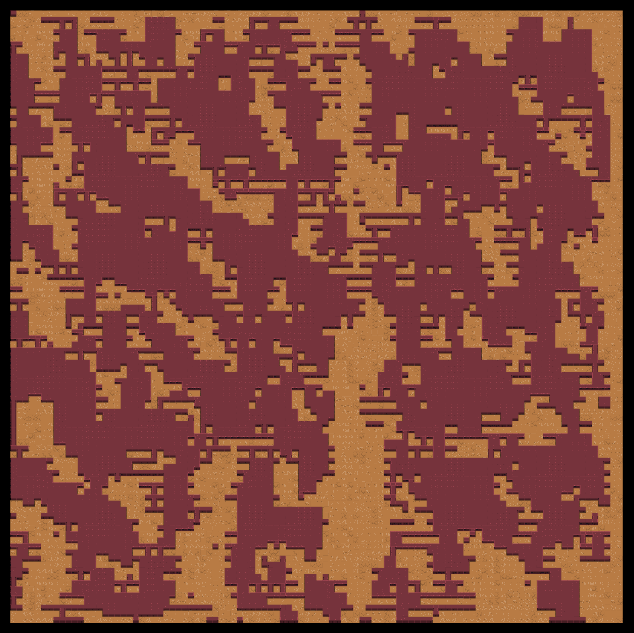
\includegraphics[width=.8\linewidth]{../images/generated/100.png}
  \caption{Επίπεδο μετά από 100 εποχές}
  \label{fig:sfig2}
\end{subfigure}
\begin{subfigure}{.5\textwidth}
  \centering
  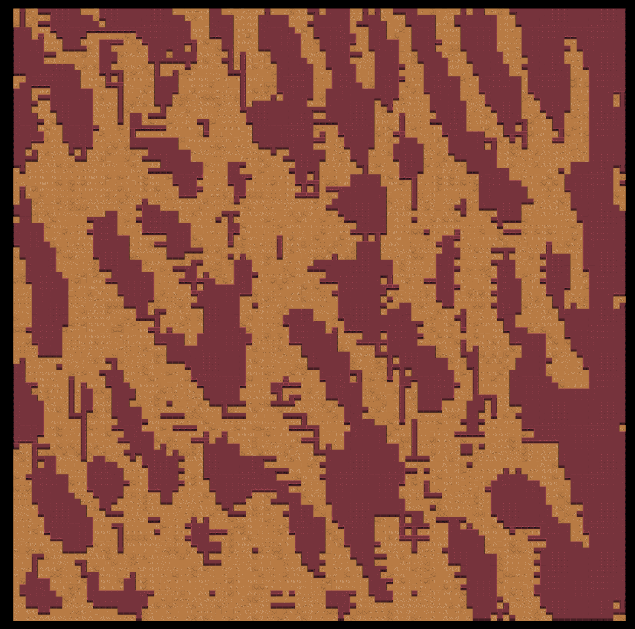
\includegraphics[width=.8\linewidth]{../images/generated/150.png}
  \caption{Επίπεδο μετά από 150 εποχές}
  \label{fig:sfig2}
\end{subfigure}
\begin{subfigure}{.5\textwidth}
  \centering
  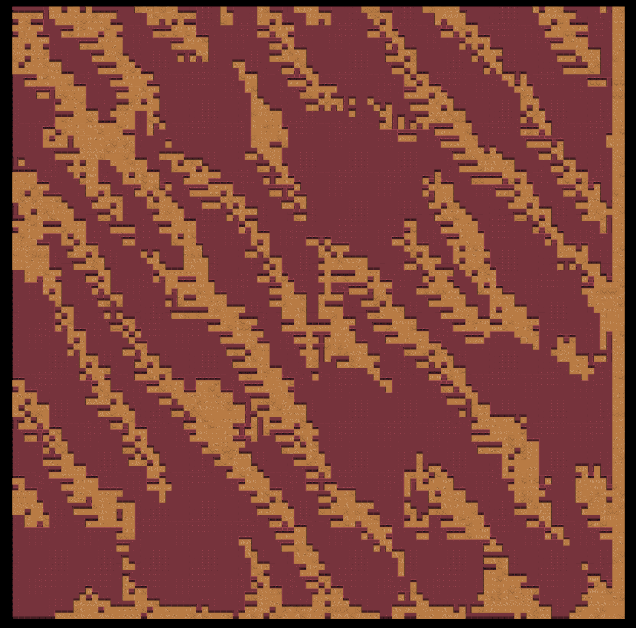
\includegraphics[width=.8\linewidth]{../images/generated/200.png}
  \caption{Επίπεδο μετά από 200 εποχές}
  \label{fig:sfig2}
\end{subfigure}
\caption{Επίπεδα που δημιούργησε κατά την εκπαίδευση των εποχών 0 - 200 το μοντέλο του GAN}
\label{fig:fig}
\end{figure}

\begin{figure}[H]
\begin{subfigure}{.5\textwidth}
  \centering
  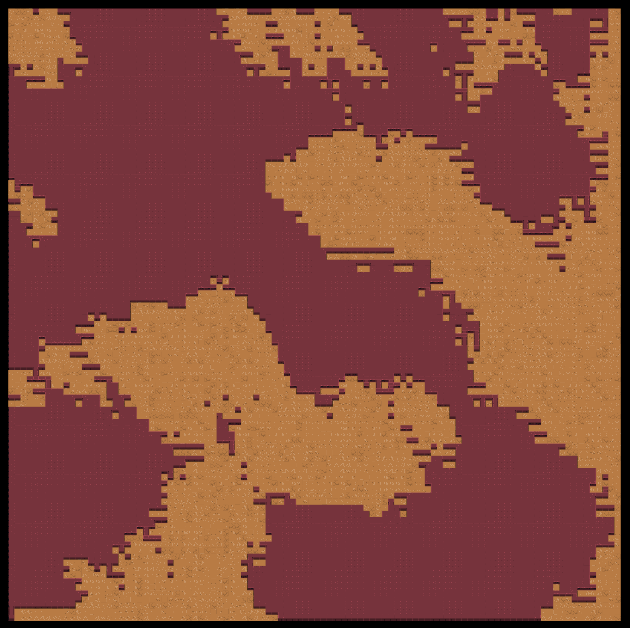
\includegraphics[width=.8\linewidth]{../images/generated/250.png}
  \caption{Επίπεδο μετά από 250 εποχές}
  \label{fig:sfig1}
\end{subfigure}%
\begin{subfigure}{.5\textwidth}
  \centering
  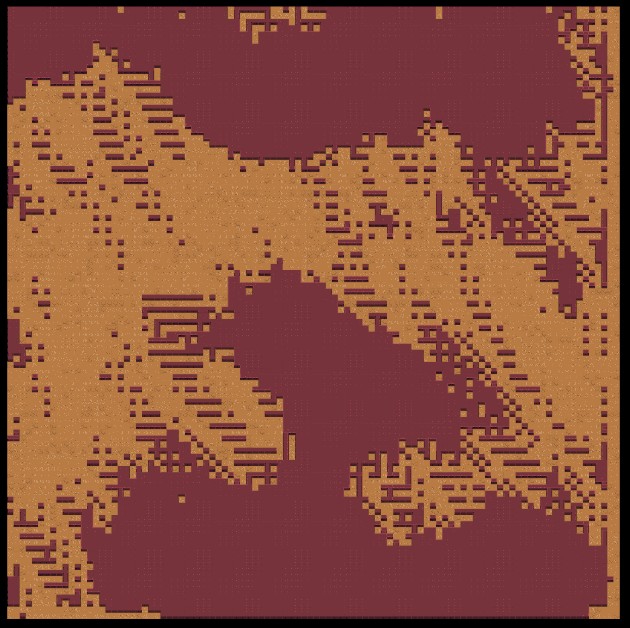
\includegraphics[width=.8\linewidth]{../images/generated/300.png}
  \caption{Επίπεδο μετά από 300 εποχές}
  \label{fig:sfig2}
\end{subfigure}
\begin{subfigure}{.5\textwidth}
  \centering
  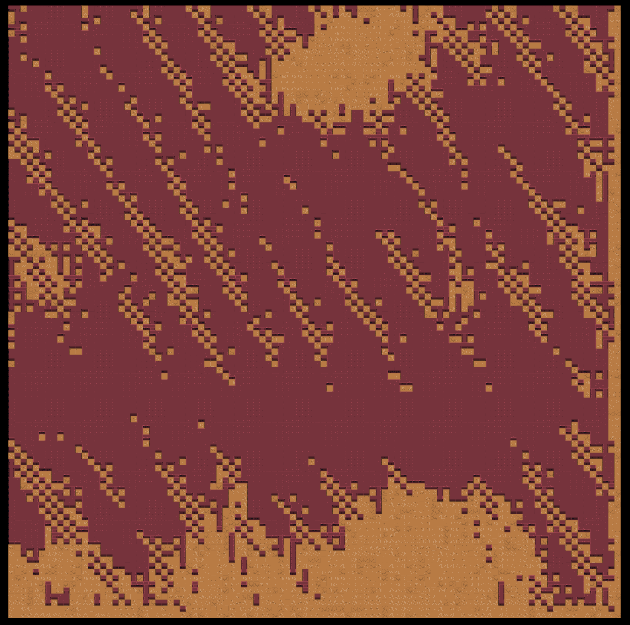
\includegraphics[width=.8\linewidth]{../images/generated/350.png}
  \caption{Επίπεδο μετά από 350 εποχές}
  \label{fig:sfig2}
\end{subfigure}
\begin{subfigure}{.5\textwidth}
  \centering
  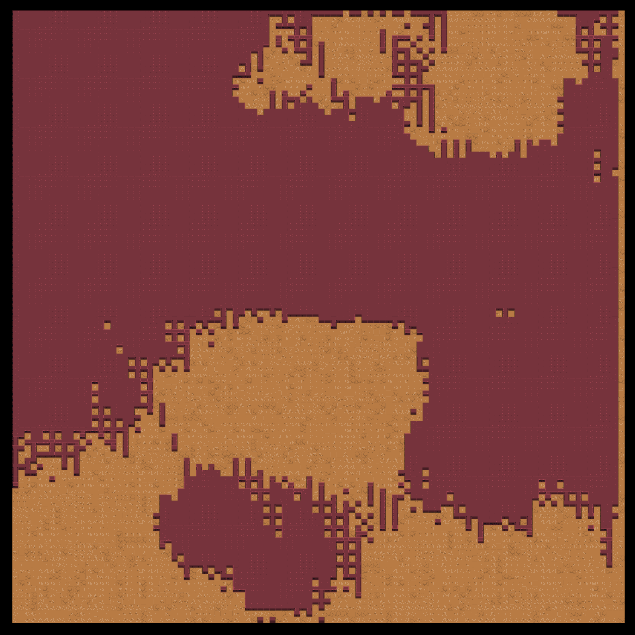
\includegraphics[width=.8\linewidth]{../images/generated/400.png}
  \caption{Επίπεδο μετά από 400 εποχές}
  \label{fig:sfig2}
\end{subfigure}
\caption{Επίπεδα που δημιούργησε κατά την εκπαίδευση των εποχών 200 - 400 το μοντέλο του GAN}
\label{fig:fig}
\end{figure}

\begin{figure}[H]
\begin{subfigure}{.5\textwidth}
  \centering
  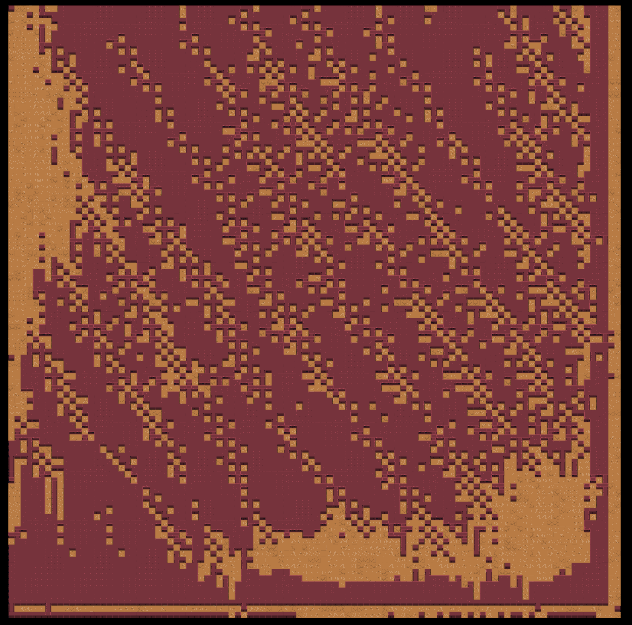
\includegraphics[width=.8\linewidth]{../images/generated/450.png}
  \caption{Επίπεδο μετά από 450 εποχές}
  \label{fig:sfig1}
\end{subfigure}%
\begin{subfigure}{.5\textwidth}
  \centering
  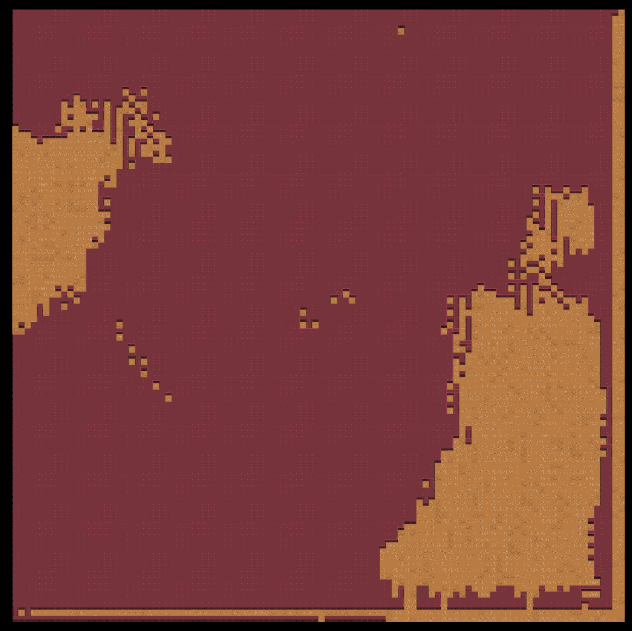
\includegraphics[width=.8\linewidth]{../images/generated/500.png}
  \caption{Επίπεδο μετά από 500 εποχές}
  \label{fig:sfig2}
\end{subfigure}
\begin{subfigure}{.5\textwidth}
  \centering
  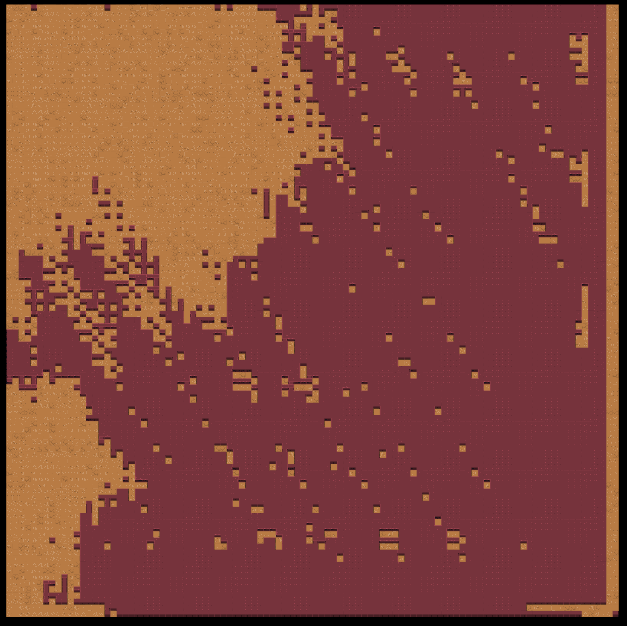
\includegraphics[width=.8\linewidth]{../images/generated/550.png}
  \caption{Επίπεδο μετά από 550 εποχές}
  \label{fig:sfig2}
\end{subfigure}
\begin{subfigure}{.5\textwidth}
  \centering
  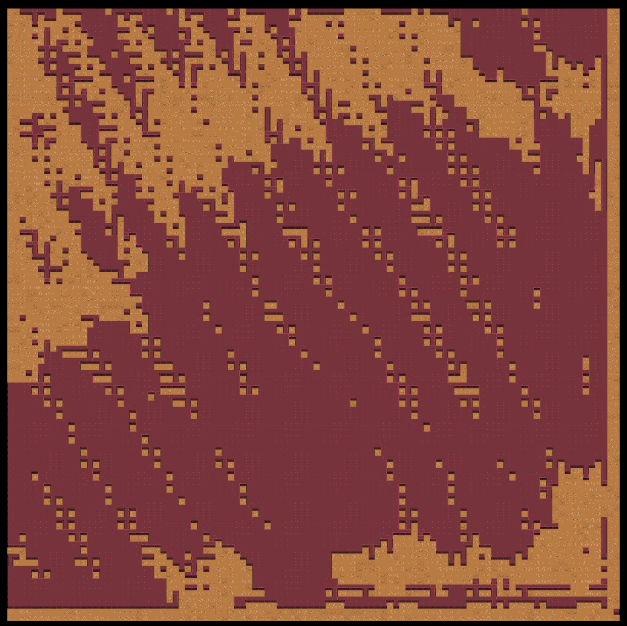
\includegraphics[width=.8\linewidth]{../images/generated/600.png}
  \caption{Επίπεδο μετά από 600 εποχές}
  \label{fig:sfig2}
\end{subfigure}
\caption{Επίπεδα που δημιούργησε κατά την εκπαίδευση των εποχών 400 - 600 το μοντέλο του GAN}
\label{fig:fig}
\end{figure}

\begin{figure}[H]
\begin{subfigure}{.5\textwidth}
  \centering
  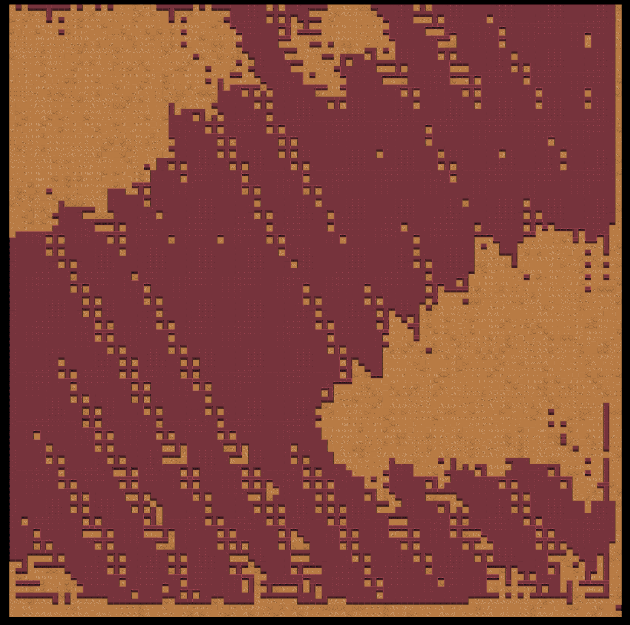
\includegraphics[width=.8\linewidth]{../images/generated/650.png}
  \caption{Επίπεδο μετά από 650 εποχές}
  \label{fig:sfig1}
\end{subfigure}%
\begin{subfigure}{.5\textwidth}
  \centering
  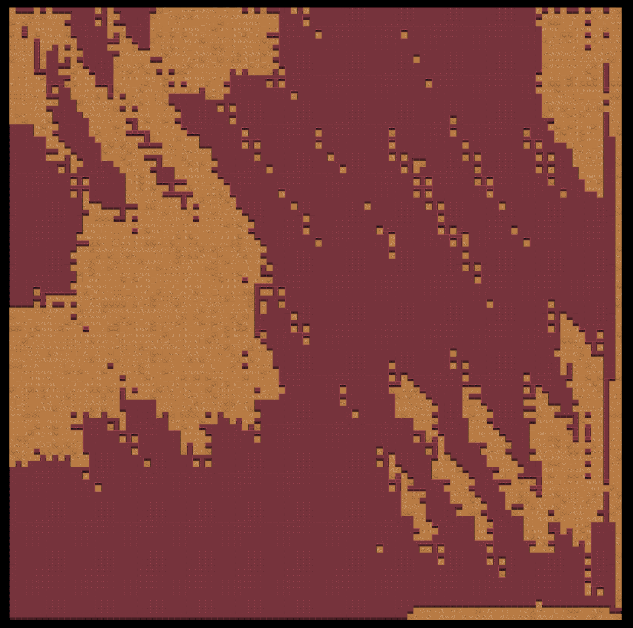
\includegraphics[width=.8\linewidth]{../images/generated/700.png}
  \caption{Επίπεδο μετά από 700 εποχές}
  \label{fig:sfig2}
\end{subfigure}
\begin{subfigure}{.5\textwidth}
  \centering
  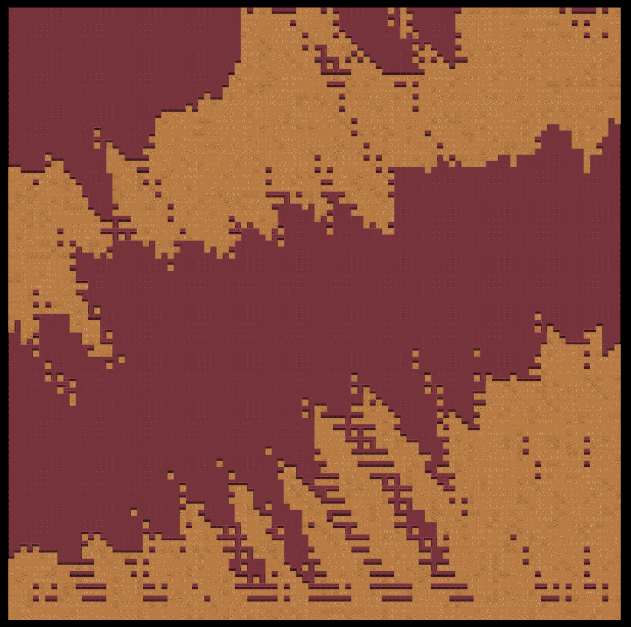
\includegraphics[width=.8\linewidth]{../images/generated/750.png}
  \caption{Επίπεδο μετά από 750 εποχές}
  \label{fig:sfig2}
\end{subfigure}
\begin{subfigure}{.5\textwidth}
  \centering
  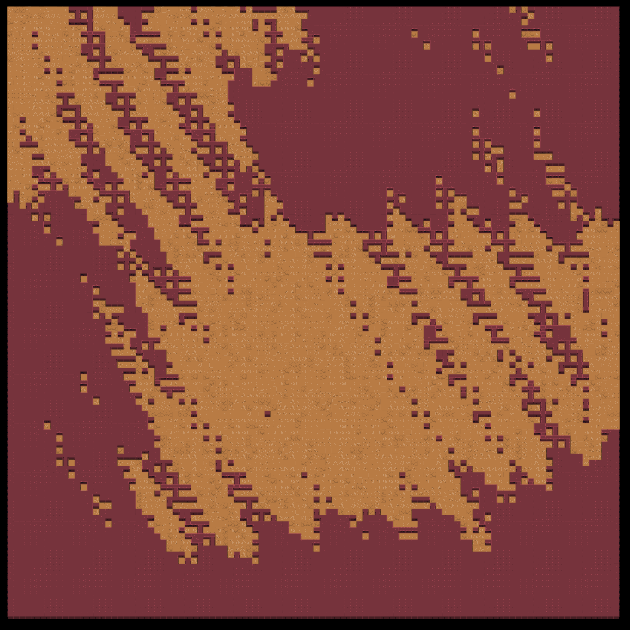
\includegraphics[width=.8\linewidth]{../images/generated/800.png}
  \caption{Επίπεδο μετά από 800 εποχές}
  \label{fig:sfig2}
\end{subfigure}
\caption{Επίπεδα που δημιούργησε κατά την εκπαίδευση των εποχών 600 - 800 το μοντέλο του GAN}
\label{fig:fig}
\end{figure}

\begin{figure}[H]
\begin{subfigure}{.5\textwidth}
  \centering
  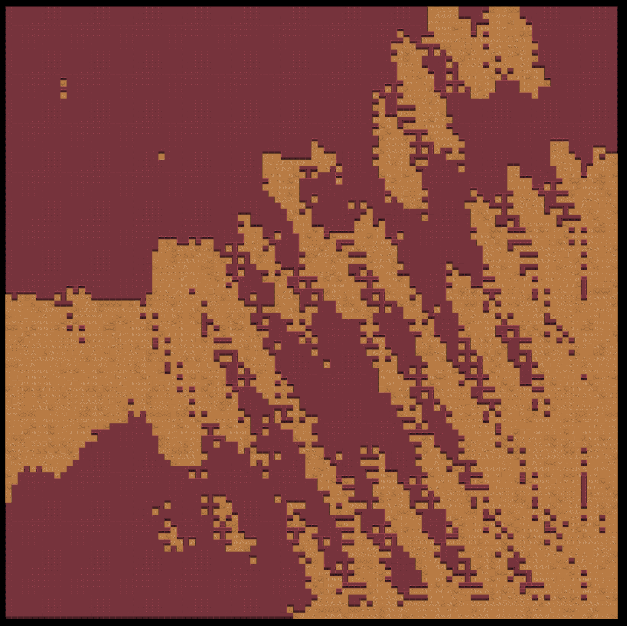
\includegraphics[width=.8\linewidth]{../images/generated/850.png}
  \caption{Επίπεδο μετά από 850 εποχές}
  \label{fig:sfig1}
\end{subfigure}%
\begin{subfigure}{.5\textwidth}
  \centering
  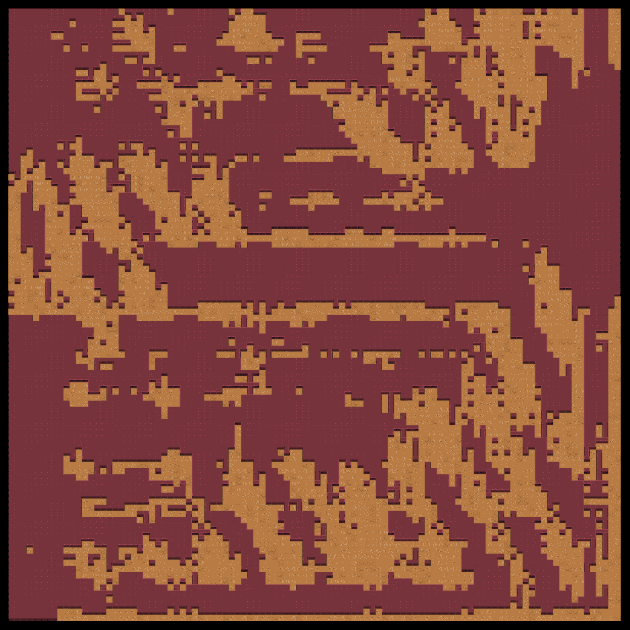
\includegraphics[width=.8\linewidth]{../images/generated/900.png}
  \caption{Επίπεδο μετά από 900 εποχές}
  \label{fig:sfig2}
\end{subfigure}
\begin{subfigure}{.5\textwidth}
  \centering
  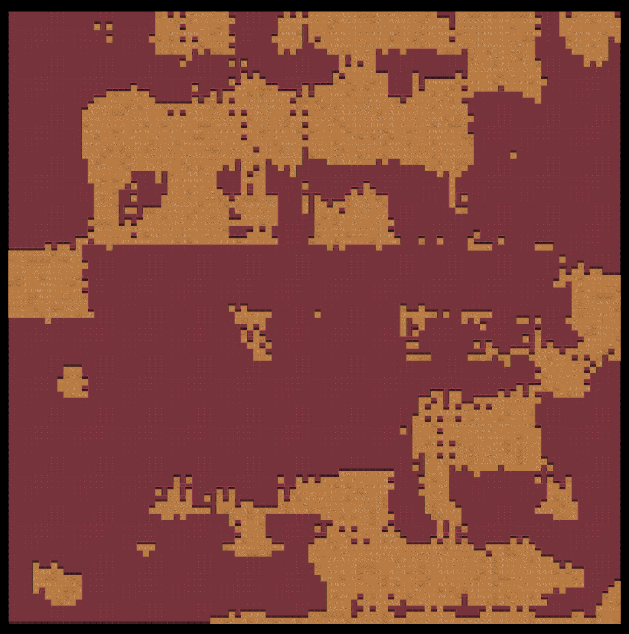
\includegraphics[width=.8\linewidth]{../images/generated/950.png}
  \caption{Επίπεδο μετά από 950 εποχές}
  \label{fig:sfig2}
\end{subfigure}
\begin{subfigure}{.5\textwidth}
  \centering
  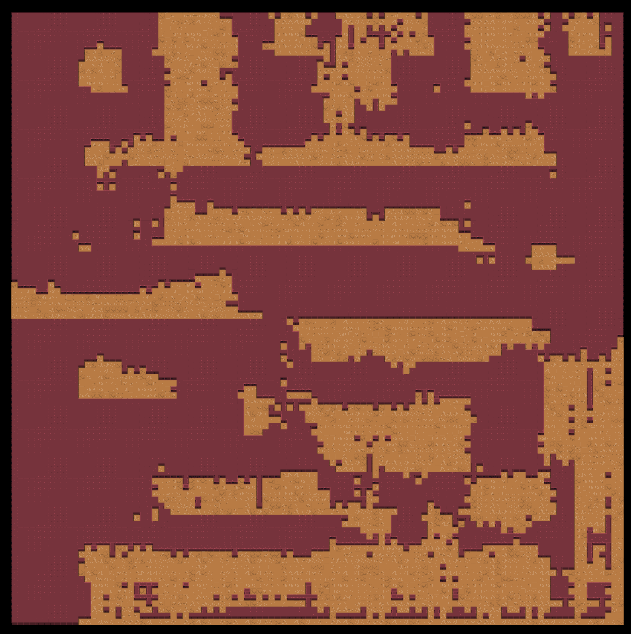
\includegraphics[width=.8\linewidth]{../images/generated/1000.png}
  \caption{Επίπεδο μετά από 1000 εποχές}
  \label{fig:sfig2}
\end{subfigure}
\caption{Επίπεδα που δημιούργησε κατά την εκπαίδευση των εποχών 800 - 1000 το μοντέλο του GAN}
\label{fig:fig}
\end{figure}

\begin{figure}[H]
\begin{subfigure}{.5\textwidth}
  \centering
  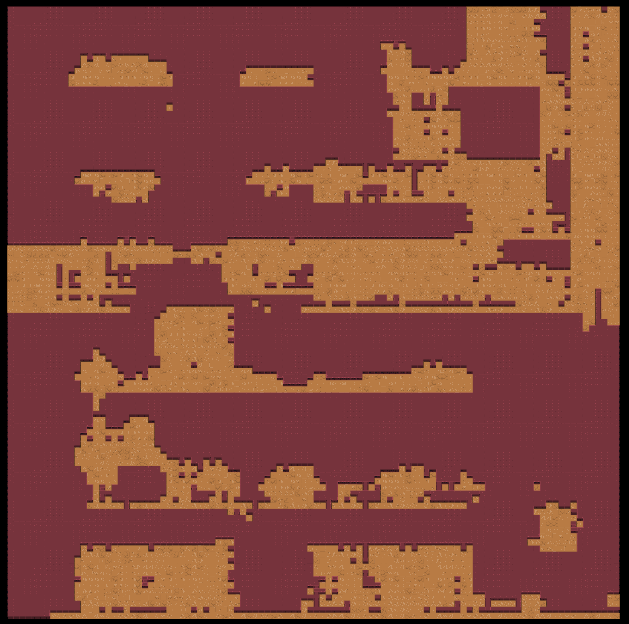
\includegraphics[width=.8\linewidth]{../images/generated/1050.png}
  \caption{Επίπεδο μετά από 1050 εποχές}
  \label{fig:sfig1}
\end{subfigure}%
\begin{subfigure}{.5\textwidth}
  \centering
  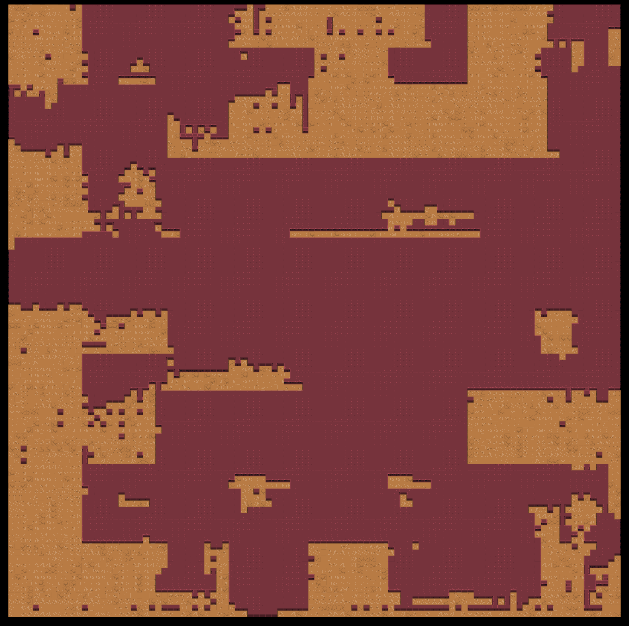
\includegraphics[width=.8\linewidth]{../images/generated/1100.png}
  \caption{Επίπεδο μετά από 1100 εποχές}
  \label{fig:sfig2}
\end{subfigure}
\begin{subfigure}{.5\textwidth}
  \centering
  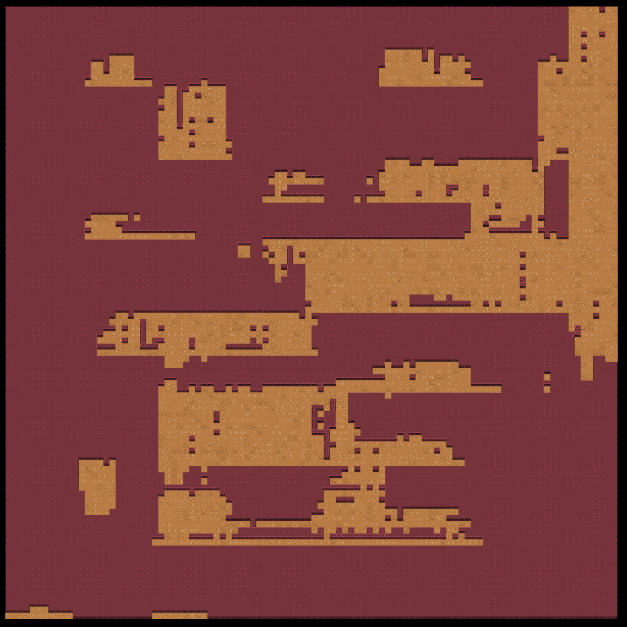
\includegraphics[width=.8\linewidth]{../images/generated/1150.png}
  \caption{Επίπεδο μετά από 1150 εποχές}
  \label{fig:sfig2}
\end{subfigure}
\begin{subfigure}{.5\textwidth}
  \centering
  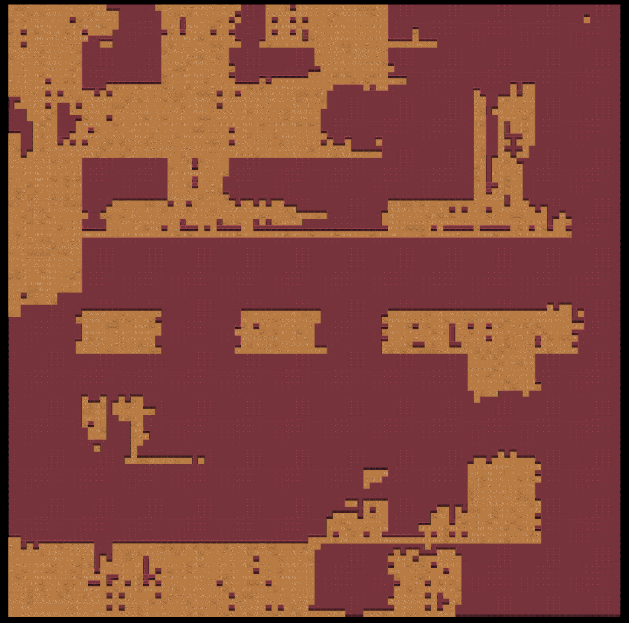
\includegraphics[width=.8\linewidth]{../images/generated/1200.png}
  \caption{Επίπεδο μετά από 1200 εποχές}
  \label{fig:sfig2}
\end{subfigure}
\caption{Επίπεδα που δημιούργησε κατά την εκπαίδευση των εποχών 1000 - 1200 το μοντέλο του GAN}
\label{fig:fig}
\end{figure}

\begin{figure}[H]
\begin{subfigure}{.5\textwidth}
  \centering
  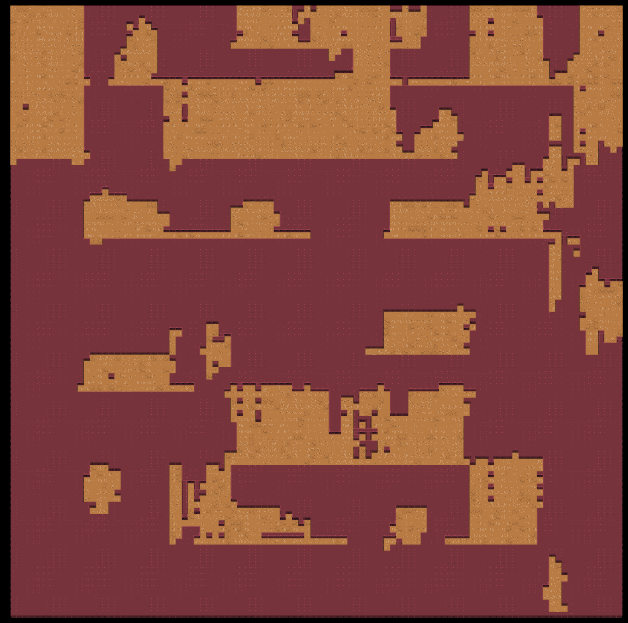
\includegraphics[width=.8\linewidth]{../images/generated/1250.png}
  \caption{Επίπεδο μετά από 1250 εποχές}
  \label{fig:sfig1}
\end{subfigure}%
\begin{subfigure}{.5\textwidth}
  \centering
  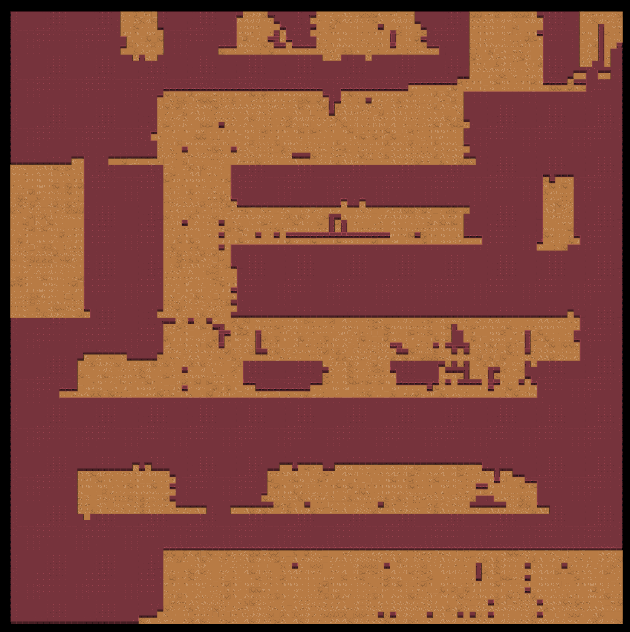
\includegraphics[width=.8\linewidth]{../images/generated/1300.png}
  \caption{Επίπεδο μετά από 1300 εποχές}
  \label{fig:sfig2}
\end{subfigure}
\begin{subfigure}{.5\textwidth}
  \centering
  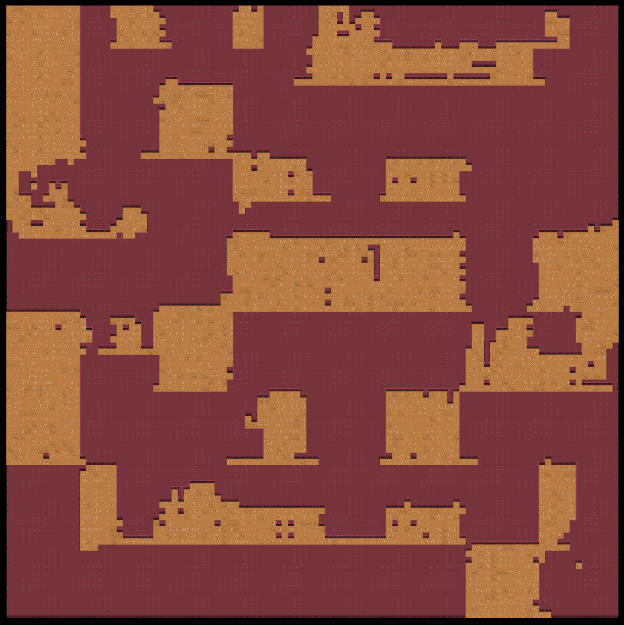
\includegraphics[width=.8\linewidth]{../images/generated/1350.png}
  \caption{Επίπεδο μετά από 1350 εποχές}
  \label{fig:sfig2}
\end{subfigure}
\begin{subfigure}{.5\textwidth}
  \centering
  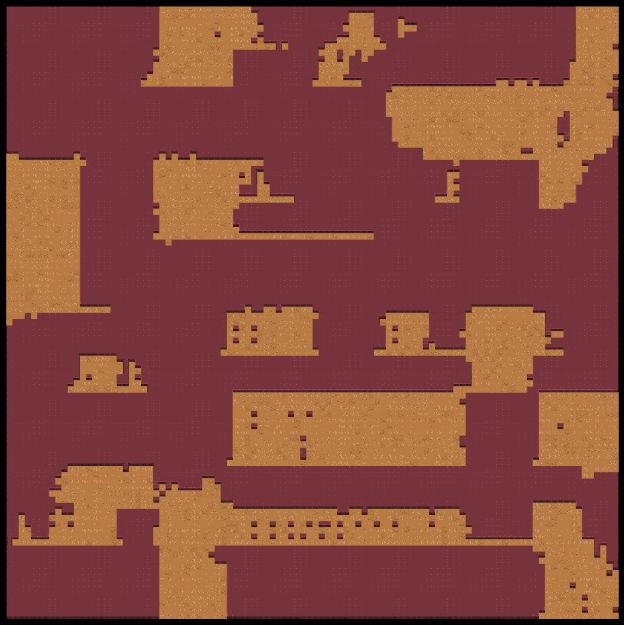
\includegraphics[width=.8\linewidth]{../images/generated/1400.png}
  \caption{Επίπεδο μετά από 1400 εποχές}
  \label{fig:sfig2}
\end{subfigure}
\caption{Επίπεδα που δημιούργησε κατά την εκπαίδευση των εποχών 1200 - 1400 το μοντέλο του GAN}
\label{fig:fig}
\end{figure}

\begin{figure}[H]
\begin{subfigure}{.5\textwidth}
  \centering
  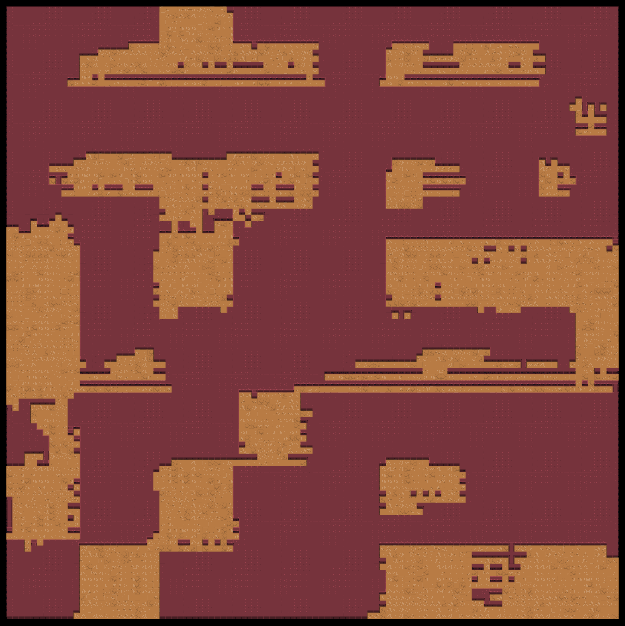
\includegraphics[width=.8\linewidth]{../images/generated/1450.png}
  \caption{Επίπεδο μετά από 1450 εποχές}
  \label{fig:sfig1}
\end{subfigure}%
\begin{subfigure}{.5\textwidth}
  \centering
  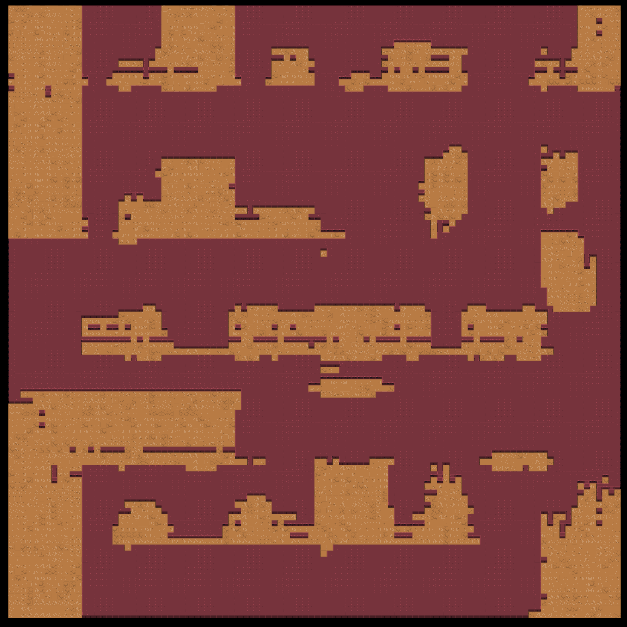
\includegraphics[width=.8\linewidth]{../images/generated/1500.png}
  \caption{Επίπεδο μετά από 1500 εποχές}
  \label{fig:sfig2}
\end{subfigure}
\begin{subfigure}{.5\textwidth}
  \centering
  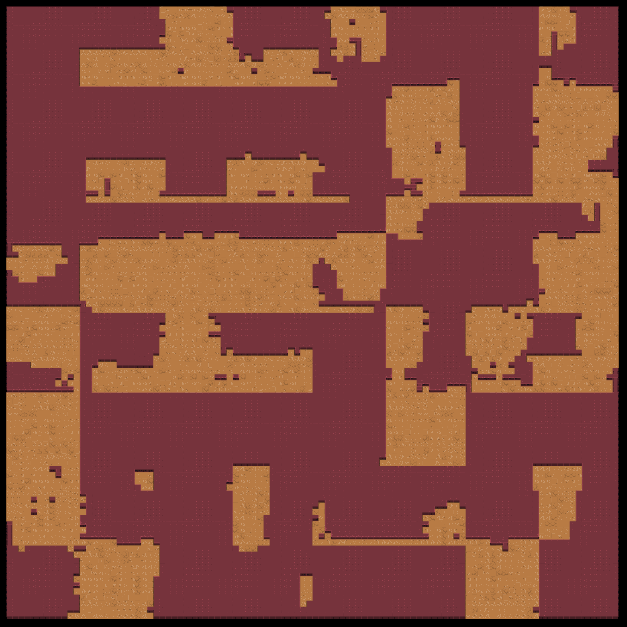
\includegraphics[width=.8\linewidth]{../images/generated/1550.png}
  \caption{Επίπεδο μετά από 1550 εποχές}
  \label{fig:sfig2}
\end{subfigure}
\begin{subfigure}{.5\textwidth}
  \centering
  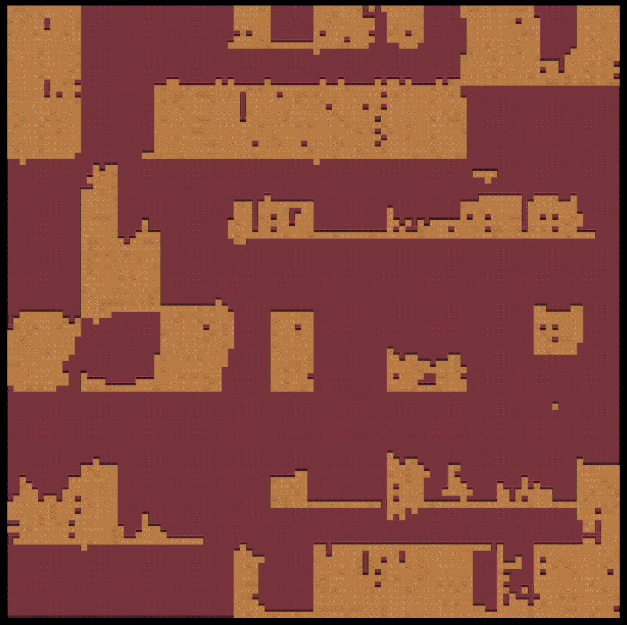
\includegraphics[width=.8\linewidth]{../images/generated/1600.png}
  \caption{Επίπεδο μετά από 1600 εποχές}
  \label{fig:sfig2}
\end{subfigure}
\caption{Επίπεδα που δημιούργησε κατά την εκπαίδευση των εποχών 1400 - 1600 το μοντέλο του GAN}
\label{fig:fig}
\end{figure}

\begin{figure}[H]
\begin{subfigure}{.5\textwidth}
  \centering
  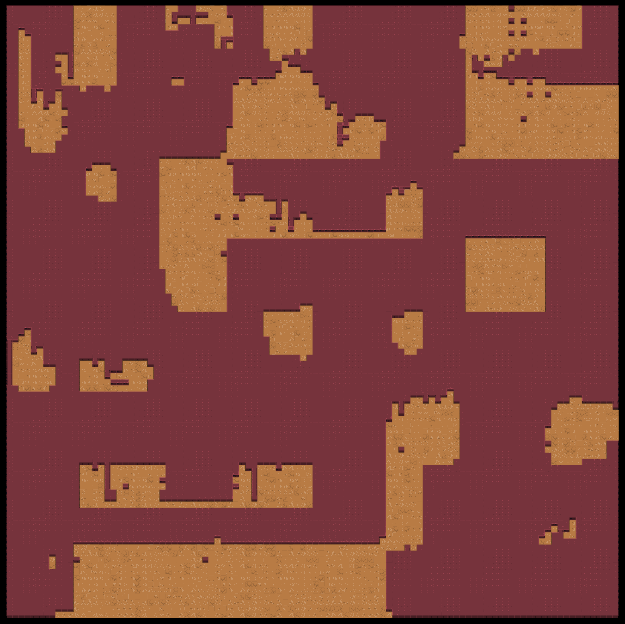
\includegraphics[width=.8\linewidth]{../images/generated/1650.png}
  \caption{Επίπεδο μετά από 1650 εποχές}
  \label{fig:sfig1}
\end{subfigure}%
\begin{subfigure}{.5\textwidth}
  \centering
  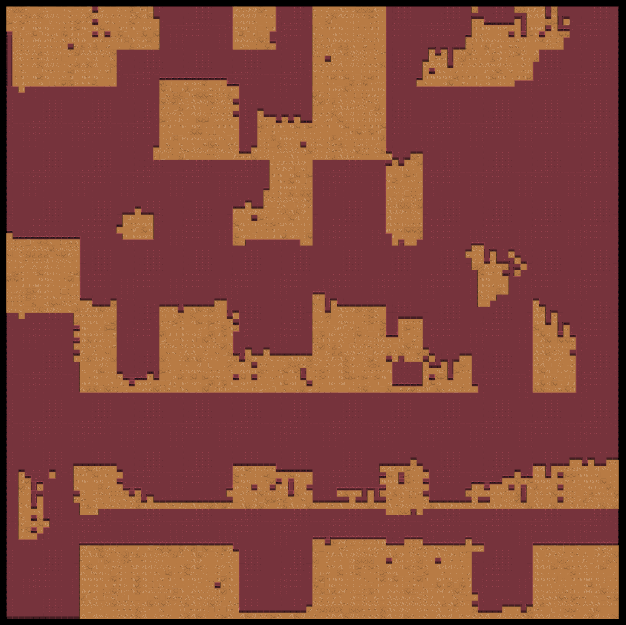
\includegraphics[width=.8\linewidth]{../images/generated/1700.png}
  \caption{Επίπεδο μετά από 1700 εποχές}
  \label{fig:sfig2}
\end{subfigure}
\begin{subfigure}{.5\textwidth}
  \centering
  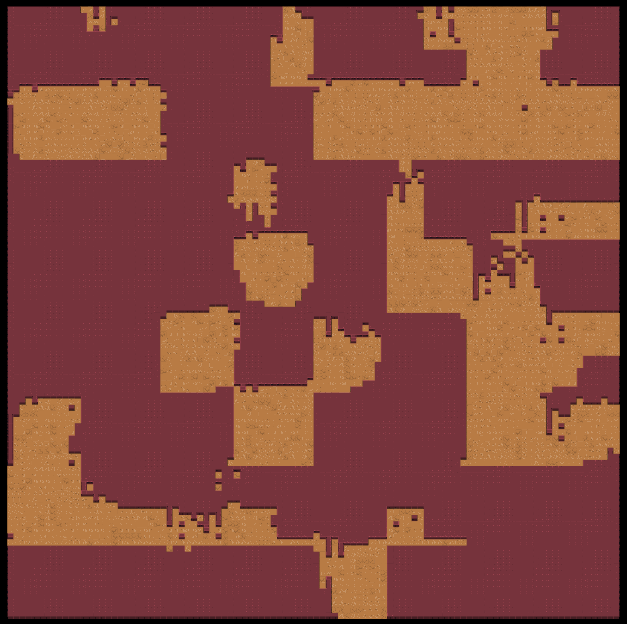
\includegraphics[width=.8\linewidth]{../images/generated/1750.png}
  \caption{Επίπεδο μετά από 1750 εποχές}
  \label{fig:sfig2}
\end{subfigure}
\begin{subfigure}{.5\textwidth}
  \centering
  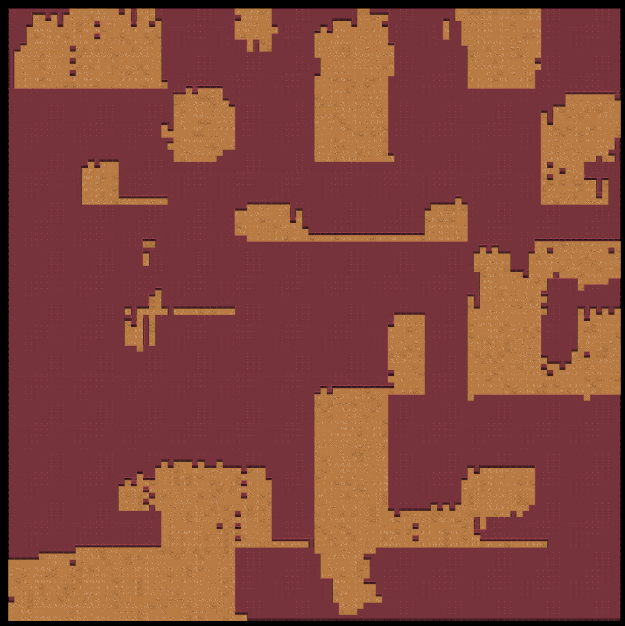
\includegraphics[width=.8\linewidth]{../images/generated/1800.png}
  \caption{Επίπεδο μετά από 1800 εποχές}
  \label{fig:sfig2}
\end{subfigure}
\caption{Επίπεδα που δημιούργησε κατά την εκπαίδευση των εποχών 1600 - 1800 το μοντέλο του GAN}
\label{fig:fig}
\end{figure}

\begin{figure}[H]
\begin{subfigure}{.5\textwidth}
  \centering
  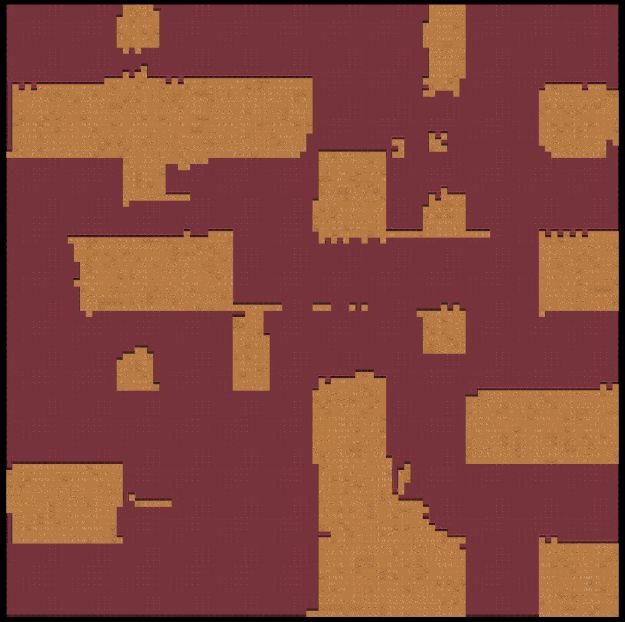
\includegraphics[width=.8\linewidth]{../images/generated/1850.png}
  \caption{Επίπεδο μετά από 1850 εποχές}
  \label{fig:sfig1}
\end{subfigure}%
\begin{subfigure}{.5\textwidth}
  \centering
  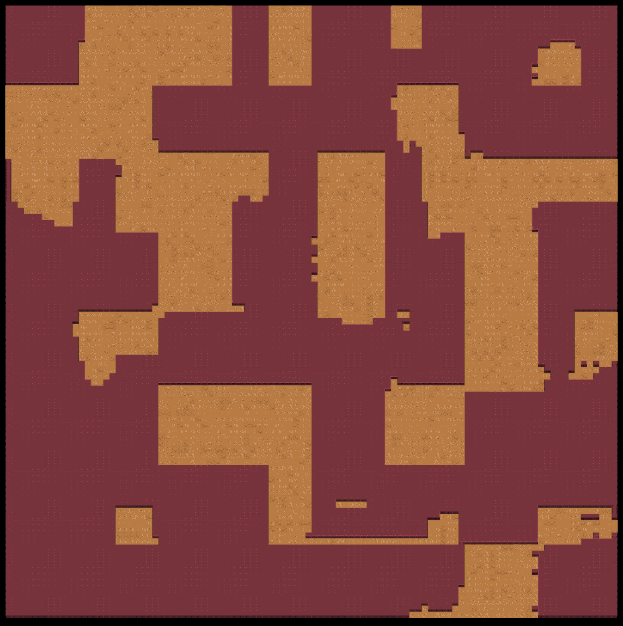
\includegraphics[width=.8\linewidth]{../images/generated/1900.png}
  \caption{Επίπεδο μετά από 1900 εποχές}
  \label{fig:sfig2}
\end{subfigure}
\begin{subfigure}{.5\textwidth}
  \centering
  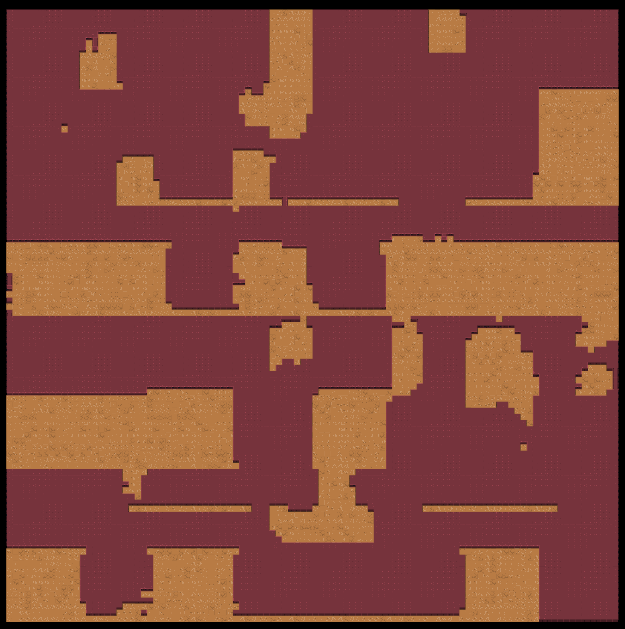
\includegraphics[width=.8\linewidth]{../images/generated/1950.png}
  \caption{Επίπεδο μετά από 1950 εποχές}
  \label{fig:sfig2}
\end{subfigure}
\begin{subfigure}{.5\textwidth}
  \centering
  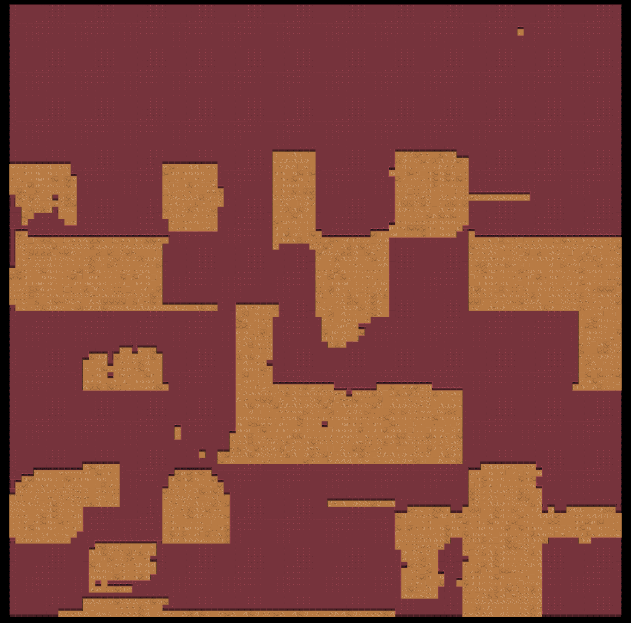
\includegraphics[width=.8\linewidth]{../images/generated/2000.png}
  \caption{Επίπεδο μετά από 2000 εποχές}
  \label{fig:sfig2}
\end{subfigure}
\caption{Επίπεδα που δημιούργησε κατά την εκπαίδευση των εποχών 1800 - 2000 το μοντέλο του GAN}
\label{fig:fig}
\end{figure}

\begin{center}
\begin{tabular}{|l|l|l|}
\hline
\textbf{Εποχή} & \textbf{Σφάλμα} & \textbf{Ακρίβεια} \\ \hline
50		   	   & 0.018495		 & 0.99\%            \\ \hline
250		       & 0.023892        & 0.98\%            \\ \hline
500  		   & 0.012442        & 0.99\%            \\ \hline
750	     	   & 0.002420        & 0.99\%            \\ \hline
1000		   & 0.026383        & 0.98\%            \\ \hline
1250		   & 0.012024        & 0.99\%            \\ \hline
1500		   & 0.098894        & 0.91\%            \\ \hline
1750		   & 0.011793        & 0.99\%            \\ \hline
2000		   & 0.009822        & 0.99\%            \\ \hline
\end{tabular}
\end{center}
\captionof{table}{Μετρήσεις σφάλματος και ακρίβειας για το μοντέλο του Discriminator} \label{tab:title}

\begin{center}
\begin{tabular}{|l|l|l|}
\hline
\textbf{Εποχή} & \textbf{Σφάλμα} & \textbf{Ακρίβεια} \\ \hline
50		   	   & 0.018495		 & 0.99\%            \\ \hline
250		       & 2.526635        & 0.22\%            \\ \hline
500  		   & 2.647155        & 0.09\%            \\ \hline
750	     	   & 6.504004        & 0.00\%            \\ \hline
1000		   & 4.416707        & 0.00\%            \\ \hline
1250		   & 5.382795        & 0.00\%            \\ \hline
1500		   & 1.574384        & 0.81\%            \\ \hline
1750		   & 6.989993        & 0.00\%            \\ \hline
2000		   & 9.392647        & 0.02\%            \\ \hline
\end{tabular}
\end{center}
\captionof{table}{Μετρήσεις σφάλματος και ακρίβειας για το μοντέλο του Generator και του Discriminator} \label{tab:title}

